\section{Grundlagen}

\begin{frame}[t]\frametitle{Gliederung: Grundlagen}
\tableofcontents[
currentsection,
subsectionstyle=show/show/hide
]
\end{frame}

\subsection{Kristallgitter}
\label{grnd:gitter}
\begin{frame}[c]\frametitle{Kristallgitter}
	Das Kristallgitter in Metallen:
	\begin{itemize}
		\item{Kubisch primitives Gitter (simple cubic)}
		\item{Kubisch raumzentriertes Gitter (body centered cubic)}
		\item{Kubisch flächenzentriertes Gitter (face centered cubic)}
	\end{itemize}
\end{frame}

\subsection{Legierungen}
\label{grnd:legierungen}
\begin{frame}[c]\frametitle{Legierung}
	Bronze (Metall-Metall Legierung).
	\begin{itemize}
		\item{Erste von Menschen genutzte Legierung.}
		\item{Kuper und Zink (CuZn)}
		\item{ca 3300v. Chr. in Palästina}
	\end{itemize}
\end{frame}

\begin{frame}[c]\frametitle{Legierung}
	Eisen
	\begin{itemize}
		\item{Wichtigste binäre Legierung Kohlenstoff}
		\item{Stahl bis 2,06\% Kohlenstoff}
		\item{Gusseisen bis 6,67\% Kohlenstoff}
	\end{itemize}
\end{frame}

\begin{frame}[c]\frametitle{Eisen-Kohlenstoff-Diagramm}
	\centering
	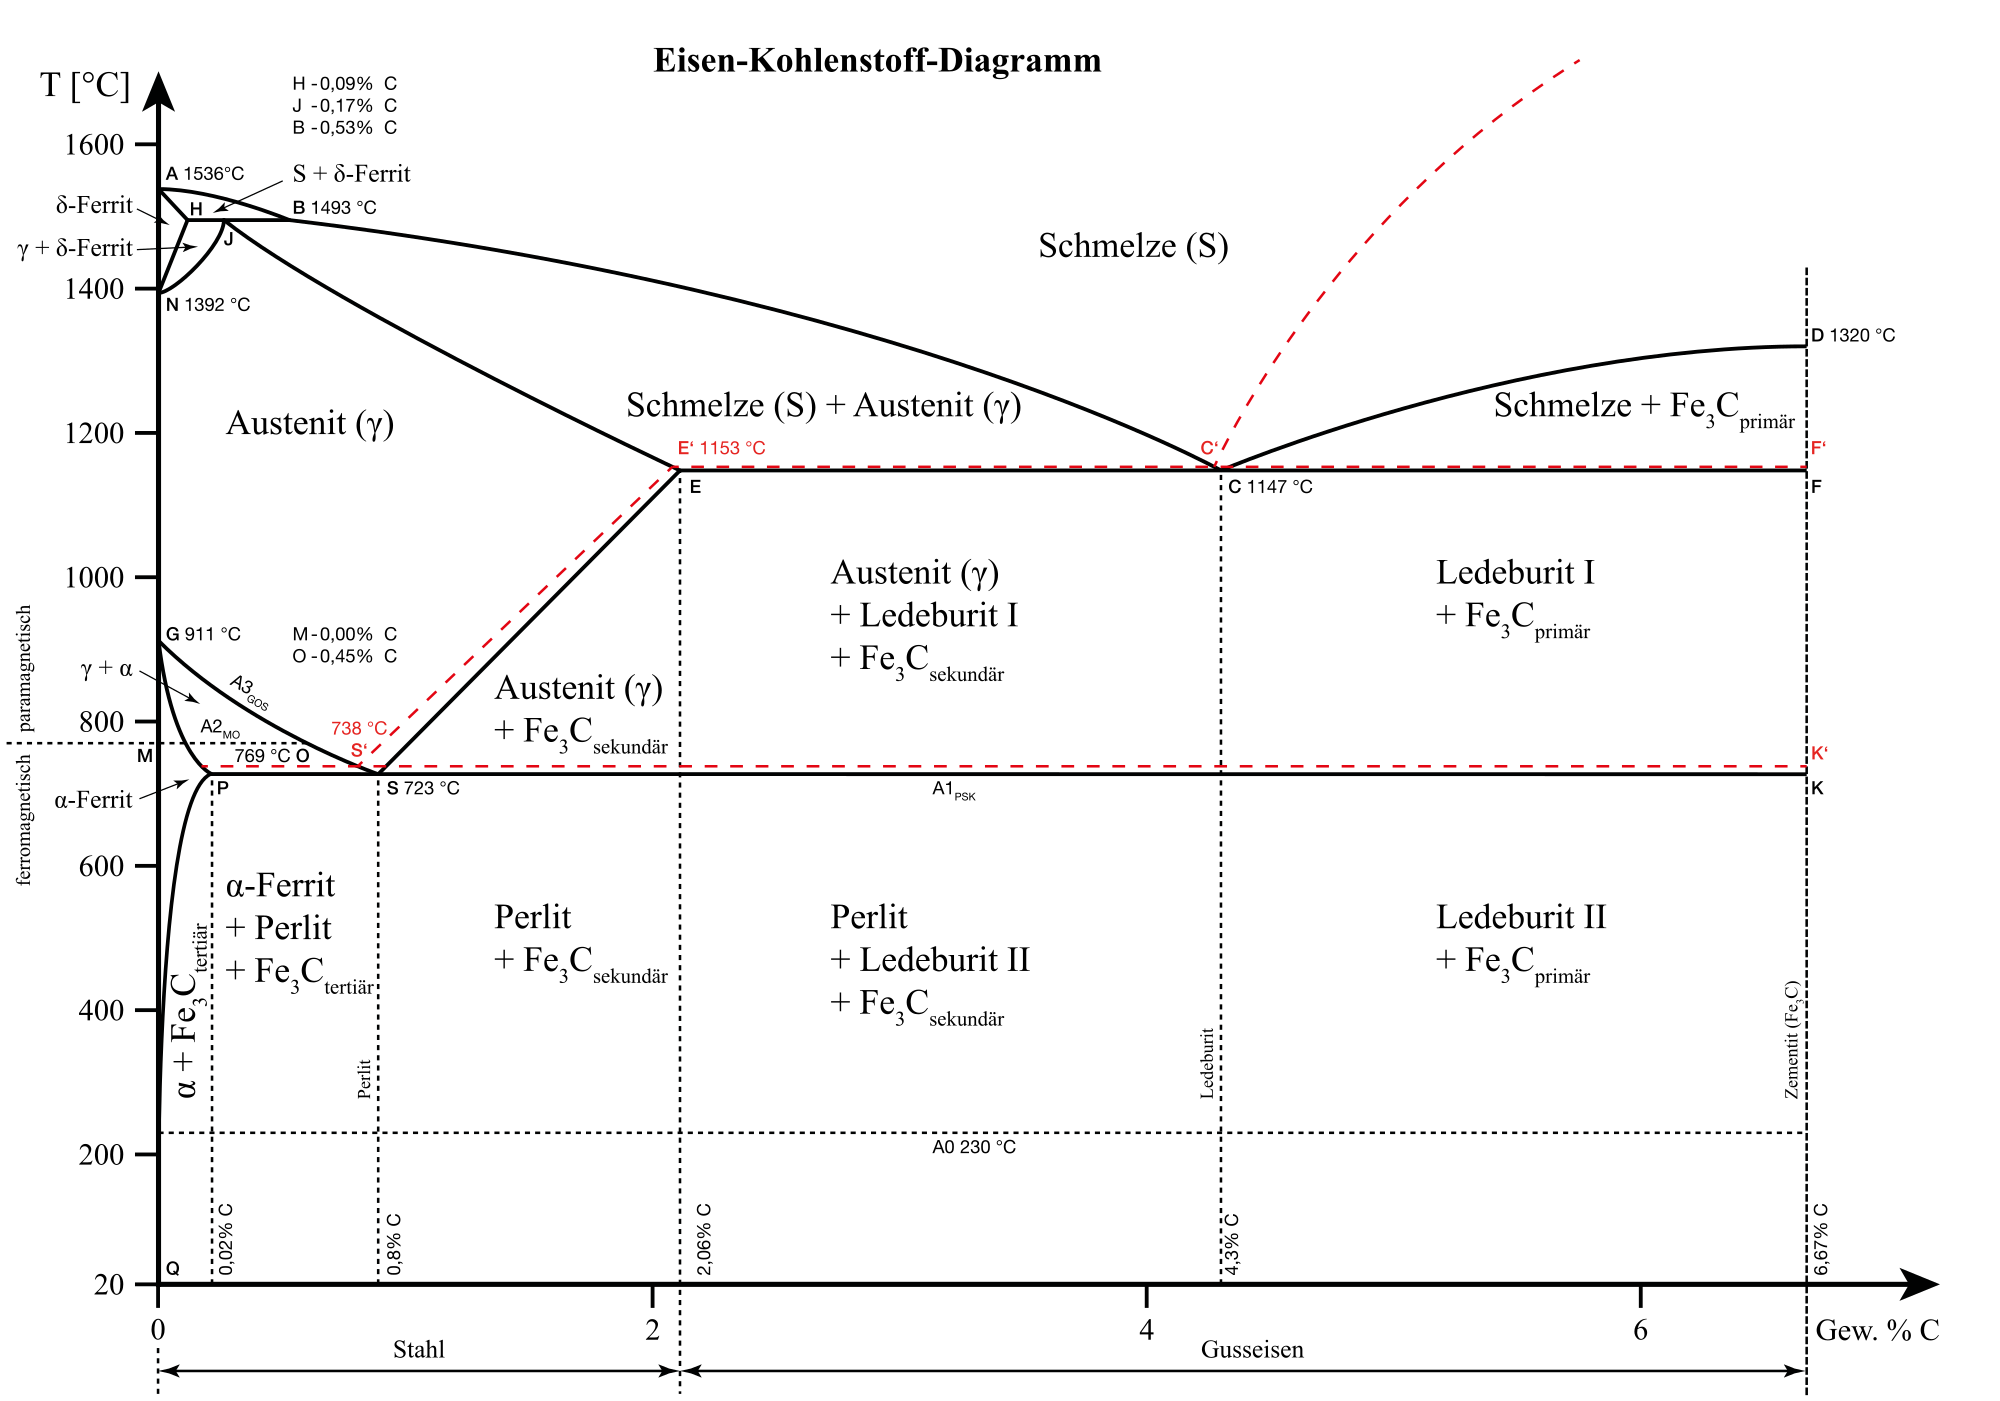
\includegraphics[height=0.5\textwidth]{medien/ekd.png}
	\\
	\tiny{Quelle:https://de.wikipedia.org/wiki/Eisen-Kohlenstoff-Diagramm}
\end{frame}
